\lhead{\emph{Evaluation}}

\chapter{Evaluation} \label{Evaluation}
\section{Experiment Setup}
\subsection{Environment}
The programming language used for this experiment is C++ to implement the algorithm and perform the single-threaded operation on an M1 pro with ten core CPU and 16GB of RAM running on a Mac Operating System. In this section, we compare four implementations mentioned in the previous section \ref{implementation}. 
The experiment will test the following trials. (1) Operation performance compares how fast it performs on read, write and update operations \textbf{Static} scenario. (2) Memory Consumption compares the amount of memory it took to perform the algorithms. (3) Number of Conflicts compares the number \conflict that happens during the insertion operations. (4) Average Tree Depth compares the number of average depths with the baseline. 
The test will perform on \textbf{Static} scenario where it assumes that the new data still follow the same distribution, and we will also test on some real-world datasets (\textbf{Dynamic} scenario) where the distribution of the new data is random. 
\subsection{Datasets}
\begin{table}
    \centering
    \begin{tabular}{ |p{2cm}|p{2cm}|p{2cm}|p{2cm}| p{2cm}|  } 
        
     \hline
     \multicolumn{5}{|c|}{Dataset} \\
     \hline
     & Gaussian Distribution & Longitudes & Log Normal & Powerlaw\\
     \hline
     \textbf{Num Keys} & 20M & 20M & 20M & 20M \\
     \textbf{Total Size} & 1.6GB & 1.6GB & 1.6GB & 1.6GB\\
     \hline
    
    \end{tabular}
     \caption{Characteristics of the dataset}
    \label{tab:characteristicdataset}
\end{table}
\subsubsection{Synthetic Datasets}
We conducted a comprehensive experimental study on synthetic datasets to evaluate the performance of different tree-based learned index implementations regarding insertion and search times. To generate the synthetic datasets, we randomly generated data based on Gaussian distribution, with the keys being of type double and 8 Bytes in size. We evaluated the different implementations based on the generated data distribution, which we characterized and analyzed. Table \ref{tab:characteristicdataset} presents the characteristics of the generated datasets.

To test the performance of the implementations, we generated a separate set of synthetic data based on the same Gaussian distribution for insertion operations. We also experimented with synthetic datasets that followed different distributions, such as power law and lognormal distributions and contained unique keys. We limit the number of keys a maximum of twenty million for simplicity in our evaluation. In the this test, we will perform bulk loading of maximum of twenty million and insertion another twenty million to test all of the operations, memory consumption and amount of new nodes creation.

A gaussian distribution, also known as a normal distribution, is a probability distribution which characterized by its symmetric and bell-shaped curved and the majority of the data is concentrated around the mean value. The gaussian distributions are commonly observed in heights of individuals in a population and etc. 

On the other hand, power law distributon is a probability distribution that follows a powerlaw, which means that the frequency of event is inversely proportional to its size raised by the constant exponent. The power law has long tail, indicating a high frequency of rare events. This distribution is commonly observed in natural such as the distribution of city sizes, the frequency of word usage and etc. 

Lastly, the lognormal distribution is characterized by a skewed, right-tailed shape, where most of the concentrated at small values. The common scenario that relates to the lognormal is the distribution of incomes and salaries.

Our experiments focused on optimizing the insertion overhead caused by \conflict that occur when space is already occupied in the tree-based learned indexes. We aimed to reduce the number of \conflict by strategically placing gaps based on the existing data distribution. This optimization is crucial, as it can significantly improve the performance of insertion operations in tree-based learned indexes.

\subsubsection{A Real World Dataset}
The Open Street Map is a comprehensive platform that provides geographic data, including longitude, which contains information about locations around the world. We have collected the longitude data from Open Street Map and used it as a basis for our dataset. Specifically, we use the longitude information as our key and test it based on an 8-byte key size \cite{openstreetmaponaws}. This data is completely random and does not follow any distribution, which accurately represents the real-world scenarios where systems insert data that may not follow any distributions.


\section{Operation Performance}
In the context of the partially sorted \learnindex and Histogram gap placement, the performance of each operation is crucial to ensure the efficiency and effectiveness of the data structure. To evaluate the performance of each operation, we measure their running time in milliseconds. Insertion, query, deletion, and adjustment are the four primary operations that we will evaluate. 

To accurately evaluate the performance of each operation, we will measure their running time in milliseconds. The running time will be measured on a variety of input sizes to ensure that the data structure can handle different workloads efficiently. Additionally, we will measure the performance of each operation under different conditions. 

By evaluating the performance of each operation, we can determine the strengths and weaknesses of the partially sorted \learnindex and Histogram gap placement and identify any areas where improvements can be made. This information will be valuable in optimizing the data structure and improving its performance in practical applications.
\subsection{Insertion}
In our recent empirical analysis, our primary objective was to comprehensively evaluate two algorithms that involve inserting partially sorted lists and gap optimization using a histogram, as compared to the baseline \acrshort{lipp} algorithm. Our overarching aim was to ascertain the extent to which these newly proposed algorithms confer a superior level of performance over the baseline and to assess the changing trend in performance compared to the baseline algorithm across different input sizes.

To achieve this aim, we subjected the algorithms to an array of tests using varying input sizes, ranging from one million to twenty million. By conducting tests across this spectrum of input sizes, we were able to determine the degree to which each algorithm's performance varied with respect to the input size.

To bolster the rigour of our assessment, we employed both static and dynamic scenarios in our evaluation. Through the use of different probability distributions, such as Gaussian, Log Normal, and Powerlaw, we sought to assess the efficacy of our algorithms in diverse and varied scenarios. Our analysis aimed to establish if the algorithms under consideration can confer a performance advantage over the baseline algorithm in these diverse scenarios.

Additionally, we conducted tests in the dynamic scenario to observe the algorithms' adaptability and robustness when dealing with random distributions. This allowed us to evaluate if the algorithms under consideration could maintain their performance gains when dealing with unforeseen circumstances.

\subsubsection{Gaussian Distribution} 
\begin{table} 
    \centering
    \begin{tabular}{ |p{2cm}|p{3cm}|p{3cm}|p{3cm}| } 
        
     \hline
     \multicolumn{4}{|c|}{Insertion Performance Result for Gaussian Distribution (in ms)} \\
     \hline
      Num Keys & Baseline (\acrshort{lipp})  & Partially Sorted & Histogram \\
     \hline
     \textbf{1M} & \cellcolor{green}106 & 150 & 136 \\
     \textbf{5M} & \cellcolor{green}696 & 845 & 742 \\
     \textbf{10M} & 1556 & 2080 & \cellcolor{green}1547 \\
     \textbf{20M} & 5875 & 7130 &\cellcolor{green} 4575 \\
     \hline
    
    \end{tabular}
     \caption{Insertion Results with Gaussian Distribution}
    \label{tab:InsertionResult}
\end{table}
\begin{figure}[H]
    \centering
    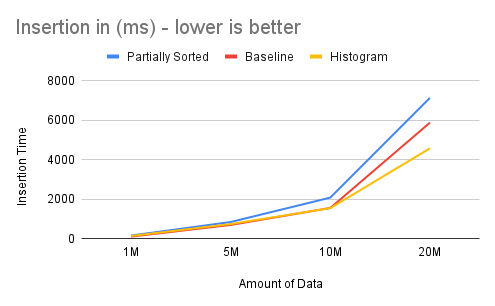
\includegraphics[width=100mm,scale=1]{Figures/InsertionResult.png}
    \caption{
Overall Insertion Operation vs Number of Insertion Operation Following Gaussian     Distribution.
    }
    \label{fig:GraphInsertionResult}
\end{figure}

The empirical analysis we conducted, which is presented in Table \ref{tab:InsertionResult} and Figure \ref{fig:GraphInsertionResult}, revealed that gap optimization using the histogram is a superior algorithm to the baseline with \acrshort{fmcd} \cite{LIPP} and partially sorted gapped array algorithms when the data follows Gaussian Distribution. This was evident from the performance gains realized by the histogram-based algorithm, which was able to capture the distribution of the data and distribute gaps based on the data's distribution, thus performing better than the \acrshort{lipp} when newly inserted data followed the same distribution as the existing data.

Moreover, the histogram-based algorithm's performance superiority over the baseline algorithm was found to widen as the amount of data stored in the \learnindex tree increased, as depicted in Figure \ref{fig:GraphInsertionResult}. This can be attributed to the histogram's efficient distribution of gaps in the data based on its distribution, which enables it to maintain optimal performance even with larger data sets.

Conversely, the partially sorted gapped array algorithm performed the worst among the three algorithms. This was mainly due to its requirement to perform a sequential search within the gapped array to locate empty spaces before inserting new data. As a result, the partially sorted algorithm's performance deteriorated as the amount of data stored in the \learnindex tree increased, as illustrated in Figure \ref{fig:GraphInsertionResult}. With larger amounts of data, there were more conflicts, which caused the partially sorted \learnindex to conduct more sequential searches, resulting in inferior performance compared to the baseline and histogram gap optimization algorithms.


\subsubsection{Lognormal Distribution}
\begin{table}
    \centering
    \begin{tabular}{ |p{2cm}|p{3cm}|p{3cm}|p{3cm}| } 
        
     \hline
     \multicolumn{4}{|c|}{Insertion Performance Result for Lognormal Distribution (in ms)} \\
     \hline
      Num Keys & Baseline (\acrshort{lipp})  & Partially Sorted & Histogram \\
     \hline
     \textbf{1M} & \cellcolor{green}127 & 156 & 199 \\
     \textbf{5M} & 1310 & 1593 & \cellcolor{green}1244 \\
     \textbf{10M} & 2593 & 3580 & \cellcolor{green}2443 \\
     \textbf{20M} & 5129 & 5930 & \cellcolor{green}4835 \\
     \hline
    
    \end{tabular}
     \caption{Insertion Results with Lognormal Distribution}
    \label{tab:InsertionResultLognormal}
\end{table}
\begin{figure}[H]
    \centering
    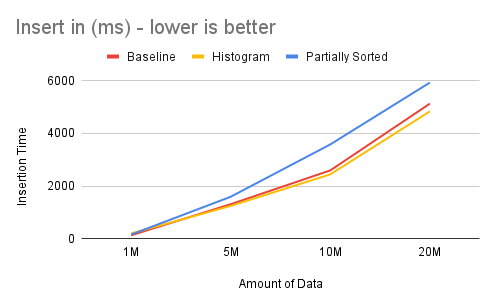
\includegraphics[width=100mm,scale=1]{Figures/InsertionResultLognormal.png}
    \caption{
     Overall Insertion Operation vs Number of Insertion Operation Following Lognormal Distribution.
    }
    \label{fig:GraphInsertionResultLognormal}
\end{figure}

Upon analyzing the results presented in Table \ref{tab:InsertionResultLognormal} and Figure \ref{fig:GraphInsertionResultLognormal}, we can conclude that the gap optimization using histogram algorithm still performs better than the baseline and partially sorted gapped array algorithms when using Log Normal Distribution. The results reveal that the histogram algorithm's superior performance is due to its ability to capture the distribution of the data and distribute gaps accordingly, thereby achieving better performance than the \acrshort{lipp} when the newly inserted data follows the same distribution as the existing data.

Similar to the findings with Gaussian Distribution, as the amount of data stored in the \learnindex tree increases, the performance gap between the histogram-based algorithm and the other two algorithms widens, as illustrated in Figure \ref{fig:GraphInsertionResultLognormal}. This can be attributed to the histogram algorithm's efficient distribution of gaps in the data, which enables it to maintain optimal performance even with larger data sets.

On the other hand, the partially sorted gapped array algorithm performed the worst among the three algorithms, as observed in the results presented in Figure \ref{fig:GraphInsertionResultLognormal}. The reason for this inferior performance can be attributed to the extra computations required to search for empty spaces after the predicted position. With larger amounts of data, the partially sorted algorithm's performance further deteriorates due to the increased amount of recursive rebuilding required when the spaces after the predicted position run out. Additionally, since each node contains more partially sorted items, each node takes longer to perform recursive rebuilding, leading to reduced performance as the amount of data increases.

The findings from our evaluation underscore the importance of considering the distribution of data when designing algorithms for processing and storing data. The results indicate that gap optimization using the histogram is a more efficient algorithm than the baseline and partially sorted gapped array algorithms, particularly when the newly inserted data follows the same distribution as the existing data. Leveraging techniques such as gap optimization using histograms can optimize performance and efficiency in data processing and storage.

\subsubsection{Powerlaw Distribution}

\begin{figure}[H]
    \centering
    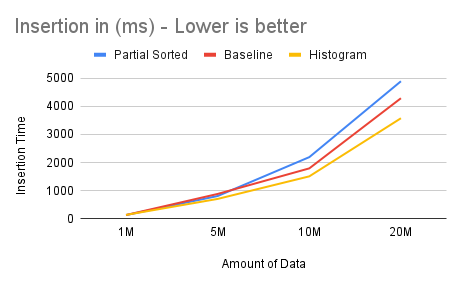
\includegraphics[width=100mm,scale=1]{Figures/InsertionResultPowerlaw.png}
    \caption{
    Overall Insertion Operation vs Number of Insertion Operation Following Powerlaw Distribution.
    }
    \label{fig:GraphInsertionResultPowerlaw}
\end{figure}
It is important to note that power-law distribution is different from the other distributions tested in that it has a long tail, meaning that there are a few elements that frequently occur while most elements are rare. This property can make it more challenging to capture the distribution using a histogram-based approach accurately.

Additionally, the wider spread of the performance gap in Figure \ref{fig:GraphInsertionResultPowerlaw} compared to the other distributions indicates that the insertion operation is more unpredictable in power-law distributed data. This may be due to the highly skewed nature of the distribution, making it difficult to predict where new elements should be inserted accurately.

Despite these challenges, the histogram-based gap optimization approach still outperforms the baseline and partially sorted gapped array in power-law distribution. This suggests that the approach is still effective in capturing the distribution and distributing gaps accordingly, leading to better insertion performance.

The poor performance of the partially sorted gapped array in power-law distribution further supports the idea that this approach is unsuitable for indexing this data type. As the amount of partially sorted keys in each node increases with larger datasets, the amount of recursive rebuilding required also increases, leading to worse performance.


\subsubsection{Real-World Dataset (Longitudes)}
\begin{figure}[H]
    \centering
    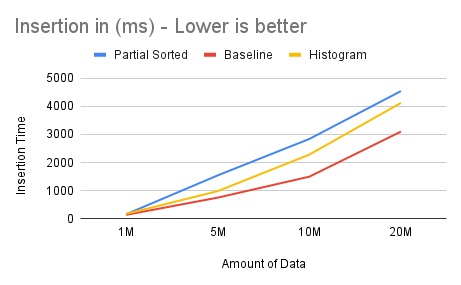
\includegraphics[width=100mm,scale=1]{Figures/InsertionResultLongitude.png}
    \caption{
       Overall Insertion Operation vs Number of Insertion Operation using Longitude Dataset.
    }
    \label{fig:GraphInsertionResultLongitude}
\end{figure}
To further analyze the result on a real-world dataset in Figure \ref{fig:GraphInsertionResultLongitude}, it is important to consider the nature of real-world data and how it can affect the performance of the algorithms. Real-world data is often diverse and can have a wide range of distributions, from uniform to skewed, and can also have varying degrees of correlation and clustering.

The baseline algorithm is able to perform better as it uses a \acrshort{fmcd} that distributes gaps and keys to optimize the linear regression model, and it does not require rebuilding during the insertion operation or does not have any assumption on the dataset. In other words, the baseline can be a good general purpose which performs well in any scenario. 

However, the histogram algorithm may not perform as well on real-world datasets as it does not account for the changing distribution of the data. The algorithm assumes that the data distribution is consistent and places gaps based on that assumption. This can lead to slower insertion times when the new data's distribution differs from the existing data.

Moreover, the partially sorted gapped array is not suitable for real-world datasets as it does not help the linear regression model improve its accuracy. Instead, it only delays the new node creation at a later stage to amortize the cost, which can be costly in terms of performance when there is a huge amount of data in the node.

The histogram algorithm is designed to work well when the distribution of the data is known, and it is able to adapt the gaps based on that distribution. But in real-world scenarios, where the distribution is not known or random, the baseline performs better as it is able to generalize to fit the randomness of the data. 

\subsection{Query}
To evaluate the performance of the query operation, we will test varying input sizes ranging from one million to twenty million, in order to determine which algorithms perform best in different scenarios and input sizes. Our tests will include both static (Gaussian, Lognormal, and Powerlaw) and dynamic (Longitudes) scenarios.

Testing static scenarios is important for query performance because it allows us to analyze the algorithms' behavior under specific data distributions. By using static datasets such as Gaussian, Lognormal and Powerlaw, we can evaluate how well the algorithms perform when the data follows a known distribution, and use this information to optimize the algorithm. For example, if an algorithm performs well on a Gaussian dataset, which is a commonly occurring distribution in real-world data, we can be confident that it will perform well on similar datasets in the future. This allows us to make more informed decisions when selecting which algorithms to use for specific tasks, and can help improve overall system performance.

Furthermore, testing static datasets allows us to measure the impact of the distribution on query performance, and identify any potential areas for optimization. This is particularly useful for algorithms that are designed to work with specific types of data distributions, such as the histogram-based algorithm that we tested earlier.

For each scenario, we will measure the query time taken by the baseline, histogram, and partially sorted algorithms. The results will be recorded and analyzed to determine which algorithm performs the best in each scenario.

This approach is necessary because different datasets may have different characteristics that affect the performance of the query operation. By testing different scenarios with varying input sizes, we can gain a better understanding of the strengths and weaknesses of each algorithm and determine which algorithm is the most suitable for a particular scenario.

Furthermore, by including both static and dynamic scenarios, we can compare the performance of the algorithms in scenarios where the data distribution is known beforehand and scenarios where the data distribution is constantly changing. This will provide valuable insights into the suitability of each algorithm in real-world scenarios where the data distribution is not known beforehand.

\subsubsection{Gaussian Distribution}
\begin{figure}[H]
    \centering
    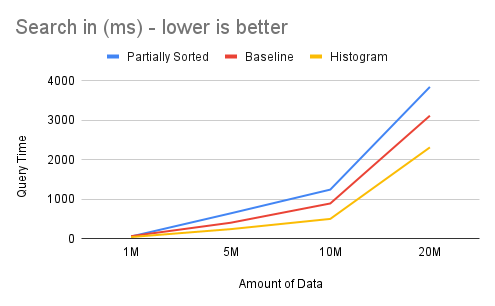
\includegraphics[width=100mm,scale=1]{Figures/QueryGaussian.png}
    \caption{
     Overall Query Operation vs Number of Query Operaton Following Gaussian Distribution
    }
    \label{fig:QueryResultGaussian}
\end{figure}
The results of the experiment show that the performance of \learnindex algorithms varies significantly depending on the distribution of the input data (Figure \ref{fig:QueryResultGaussian}). When it comes to query operations on the Gaussian Distribution, the histogram algorithm outperforms the other algorithms. This is because the histogram algorithm makes use of the gaps between keys that are specifically optimized for the given distribution. By doing so, it traverses lesser depth, which in turn improves the overall query performance.

On the other hand, the baseline algorithm performs relatively well compared to the partially sorted \learnindex algorithm. However, the baseline algorithm tries to generalize and perform well in most cases without taking advantage of the prior data distribution. This means its performance is less than the histogram algorithm in certain distribution types.

The partially sorted algorithm performs the worst of the other two algorithms in query operations. This is due to the extra computational overhead required when the keys are partially sorted. Even though the amount of conflicts is reduced with the partially sorted gapped array, the algorithm still spends a significant amount of time doing sequential searches due to potential miss predictions by the model and the partially sorted gapped array.

It is important to note that the above results were obtained in static scenarios, where the input data distribution remains constant. The histogram algorithm performed best in static scenarios because it was specifically optimized for the given distribution. 

\subsubsection{Lognormal Distribution}
\begin{figure}[H]
    \centering
    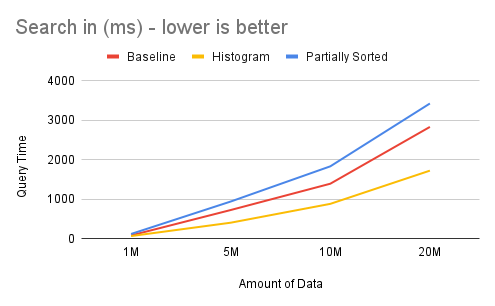
\includegraphics[width=100mm,scale=1]{Figures/QueryLognormal.png}
    \caption{
     Overall Query Operation vs Number of Query Operation Following Lognormal Distribution.
    }
    \label{fig:QueryResultLognormal}
\end{figure}
The experiment was also conducted on a lognormal distribution dataset. Similar to the Gaussian distribution (Figure \ref{fig:QueryResultLognormal}), the histogram algorithm outperformed the baseline \acrshort{lipp} and the partially sorted array in terms of query performance. The results shown in Figure 2 demonstrate that as the amount of data increases, the performance gap between the histogram and the baseline widens. This indicates that the histogram algorithm takes advantage of the data distribution and optimizes gaps in a way that allows the query to traverse fewer levels in the tree, leading to better performance.

On the other hand, the baseline algorithm still outperformed the partially sorted array even though the latter had a lower average tree depth. This is due to the extra computational overhead required for the $\epsilon$ linear search when there are a large number of partially sorted items in the tree. Despite having a lower average tree depth, the partially sorted array's slower search process prevented it from performing as well as the baseline in terms of query performance.

\subsubsection{Powerlaw Distribution}
\begin{figure}[H]
    \centering
    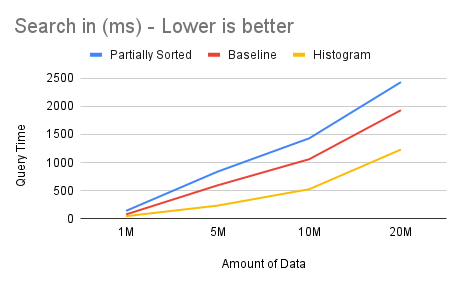
\includegraphics[width=100mm,scale=1]{Figures/QueryPowerlaw.png}
    \caption{
Overall Query Operation vs Number of Query Operation Following Powerlaw Distribution.
    }
    \label{fig:QueryResultPowerlaw}
\end{figure}
The study also evaluated the performance of the three data structures on Zipfian distribution (Figure \ref{fig:QueryResultPowerlaw}). The results were similar to the other distributions, with the histogram performing the best and the partially sorted gapped array performing the worst.

The histogram data structure again outperformed the baseline and partially sorted \learnindex structures due to its optimization for the Zipfian distribution. The gaps in the histogram structure are also specifically designed to account for the high frequency of certain keys in the distribution, resulting in a lower average tree depth and improved query performance.

In contrast, the baseline \learnindex performed relatively well in querying Zipfian distribution, but still could not match the efficiency of the histogram. This is because the baseline tries to generalize and perform well in most cases, but does not take full advantage of the specific distribution characteristics.

The partially sorted gapped array again struggled with the Zipfian distribution, with the extra computational overhead of the $\epsilon$ linear search causing a significant performance gap from the other two structures. As with the other distributions, the partially sorted \learnindex performed better than the baseline \learnindex in terms of average tree depth. However, this improvement was outweighed by the increased search time from the linear search.

\subsubsection{Real-World Dataset (Longitudes)}
\begin{figure}[H]
    \centering
    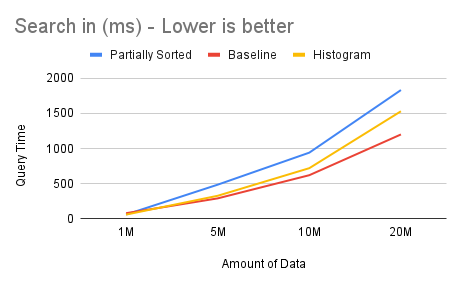
\includegraphics[width=100mm,scale=1]{Figures/QueryLongitude.png}
    \caption{
     Overall Query Operation vs Number of Query Operation using Longitude Dataset.
    }
    \label{fig:QueryResultLongitude}
\end{figure}
Moving to a real-world dataset, the experimental result in Figure \ref{fig:QueryResultLongitude} shows that the histogram performs on par with the baseline when it comes to range query. This indicates that both the baseline and histogram have a similar average tree depth which contributes to the similar query performance.

It is important to note that the query performance is heavily dependent on the height of the tree. If the tree height is greater, it leads to poor query performance. This can be attributed to the fact that a larger height would require the query algorithm to traverse through more levels of the tree, hence making the query more time-consuming.

However, when it comes to the partially sorted gapped array, the performance is still not up to the mark. Despite having a lower average tree depth compared to both baseline and histogram, the extra computation required for the linear search, after traversing the tree depth, hampers its overall query performance.


\subsection{Deletion}
In order to gain a deeper understanding of the performance of partially sorted and histograms compared to the baseline, we conduct further experiments involving delete operations. This setup is similar to the previous tests, with varying input sizes ranging from one to twenty million, using different distributions and a real-world dataset.

In the deletion operation, the performance is expected to be similar to that of the query operation, as the tree must be traversed to locate the keys before they can be deleted. This provides us with additional insight into the efficiency of each algorithm and how they handle deletions.

These experiments will allow us to further analyze the performance of each algorithm in different scenarios, providing a more comprehensive understanding of their strengths and weaknesses.

\subsubsection{Gaussian Distribution}
\begin{figure}[H]
    \centering
    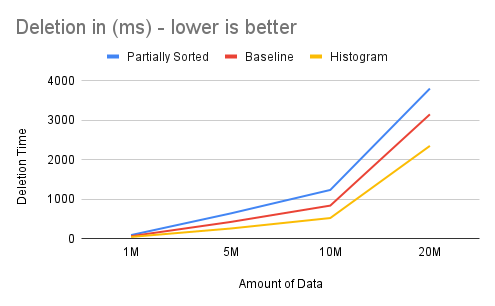
\includegraphics[width=100mm,scale=1]{Figures/DeleteGaussian.png}
    \caption{
Overall Deletion Operation vs Number of Deletion Operation Following Gaussian     Distribution.    }
    \label{fig:DeleteGaussian}
\end{figure}
The results Figure \ref{fig:DeleteGaussian} showed that the histogram outperformed both the baseline and the partially sorted array in Gaussian distribution. This was due to the lesser average depth of the tree, which made traversing down the tree faster, allowing for faster deletions.

It was also observed that the baseline still performed better than the partially sorted, even though it had a higher average tree depth compared to the partially sorted array. This was due to the precise position of the keys from the model and not requiring an extra linear search like the partially sorted gapped array. Furthermore, the sharp spike is due to increasing data from 10 M to 20 M.


\subsubsection{Powerlaw Distribution}
\begin{figure}[H]
    \centering
    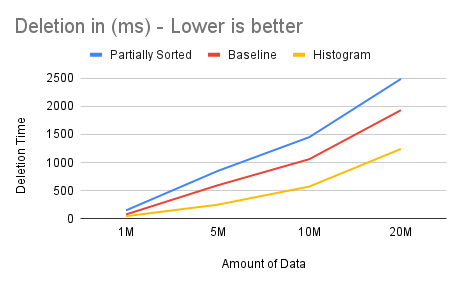
\includegraphics[width=100mm,scale=1]{Figures/DeletePowerlaw.png}
    \caption{
Overall Deletion Operation vs Number of Deletion Operation Following Powerlaw Distribution.
    }
    \label{fig:DeletePowerlaw}
\end{figure}
For the Powerlaw Distribution, we use a similar strategy as other distributions where we bulk load the keys and then insert the same amount into the tree. The resulting Figure \ref{fig:DeletePowerlaw} shows that the histogram still outperforms both baseline and partially sorted. The deletion works similarly to the query as it has to traverse down until it reaches a key before performing deletion which makes the deletion process bounded by the height of the tree. In this case, the reason why histogram achieve better performance is because it is able to make use of the gaps available in upper node and create lesser child node than the baseline. However partially sorted is slower even with similar tree depth is because it is bounded by the $\epsilon$ spaces and the height of the tree. The amount of time is mostly spent on the linear $\epsilon$ search which causes the gap in performance between the histogram and the partially sorted. 


Overall, the results in Figure \ref{fig:DeletePowerlaw} showed that the histogram indexing algorithm was consistently the best performer in terms of query, insertion, and deletion operations across various distributions and real-world datasets. However, it is worth noting that the baseline algorithm also performed relatively well and could be considered as a viable alternative in scenarios where the data distribution is unknown. On the other hand, the partially sorted gapped array algorithm performed poorly and could be improved by reducing the number of partially sorted keys in the gapped array.


\subsubsection{Real-World Dataset (Longitudes)}
\begin{figure}[H]
    \centering
    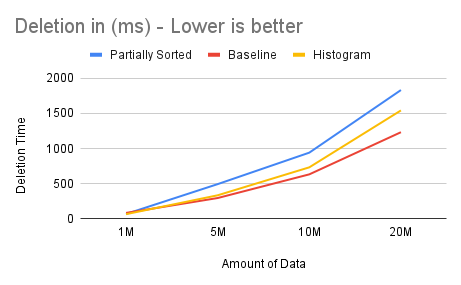
\includegraphics[width=100mm,scale=1]{Figures/DeleteLongitude.png}
    \caption{
    Overall Deletion Operation vs Number of Deletion Operation using Longitude Dataset.
    }
    \label{fig:DeleteLongitude}
\end{figure}
The real-world dataset serves as a more practical and relevant evaluation for these algorithms. The deletion operation is expected to have a similar performance to the query operation since both require traversing down the tree to locate the keys to be deleted or queriesd. As expected, the results in Figure \ref{fig:DeleteLongitude} show that the histogram and baseline perform similarly when deleting keys from the tree. This is due to their similar number of average tree height, which is a crucial factor that influences the query or deletion performance.

In contrast, the partially sorted gapped array performs worse than the histogram and baseline. Even though the partially sorted array has a lower average tree depth than the baseline, it requires an extra linear search after traversing down the tree to search for the predicted position of the key. This search is necessary because the keys could be located anywhere within a range of $x$ to $x + \epsilon$ around the predicted position. Consequently, the partially sorted array is bounded by the tree's height and the $\epsilon$ limit spaces after the predicted position. These factors contribute to its inferior performance compared to the histogram and baseline.


\subsection{Adjustment / Branch Pruning}
\begin{figure}[H]
    \centering
    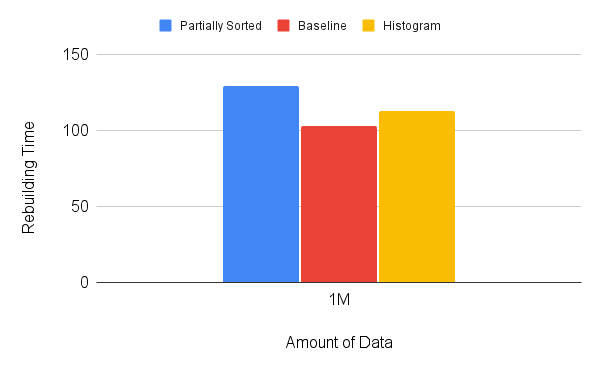
\includegraphics[width=100mm,scale=1]{Figures/RebuildingGaussian.png}
    \caption{
     Overall Rebuilding Time vs Amount of Keys in the Tree Following Gaussian Distribution
    }
    \label{fig:RebuildingGaussian}
\end{figure}
The \acrfull{lipp} algorithm is designed to optimize the performance of learned indexes by making adjustments to the tree's structure under specific conditions. These adjustments aim to reduce the tree's height, thereby reducing the time it takes to access and retrieve keys. During our testing of the learned indexes, we did not modify any of these conditions since they were already optimized for performance. However, we recognized that each of the algorithms (baseline, histogram, and partially sorted) has a unique implementation of these adjustments, which needed to be tested to determine the most effective implementation.

To test the effectiveness of these adjustments, we employed a rigorous testing strategy. We tested the algorithms on the Gaussian distribution dataset and measured the execution time in milliseconds. By comparing the performance of the three algorithms, we aimed to identify which implementation of the adjustments was most effective.

From the result Figure \ref{fig:RebuildingGaussian}, we observed that the histograms perform slower than the baseline on the test data. This is because the gap redistribution, retraining of the model, and rebuilding new histogram from the newly collected keys required for the histogram adjustments result in an operating cost of $O(N\log N)$. It costs the same as the baseline $O(N\log N)$ \cite{LIPP}, but the baseline does not need to rebuild the histogram, making it faster than the histogram algorithm. The partially sorted algorithm also performed worse than the baseline and histogram algorithms. This can be attributed to the challenges associated with collecting partially sorted keys. Nevertheless, like the histogram algorithm, the partially sorted algorithm's adjustments were also dominated by the retraining of the model and the collection of keys.



\section{Memory Consumption}
In addition to measuring the execution time, it is also essential to analyze the memory consumption of each implementation. Memory consumption refers to the amount of memory that is required to perform each operation. Therefore, in this section, we will be using the same data set as before but measuring the memory consumption of each implementation.

Measuring memory consumption is crucial as it helps us determine the amount of memory resources required to run each algorithm effectively. By analyzing the memory consumption, we can optimize the algorithm to reduce its memory footprint, which is important in scenarios where memory is a scarce resource.

We will use the same testing strategy as before, running each algorithm on the same data set and measuring the memory consumption in bytes. By comparing the memory consumption of the three algorithms, we can determine which implementation is the most memory-efficient.

It is important to note that memory consumption is affected by various factors, such as the size of the data set, the structure of  the data, and the algorithm's implementation. Therefore, the results obtained in this section will provide valuable insights into the memory consumption of each algorithm and help us optimize the algorithm for better performance.

\subsection{Gaussian Distribution}
\begin{figure}[H]
    \centering
    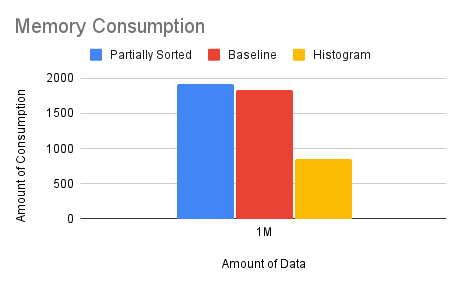
\includegraphics[width=100mm,scale=1]{Figures/MemoryGaussian.png}
    \caption{
     Results of Memory Consumption with Gaussian Dataset 1M
    }
    \label{fig:MemoryGaussian}
\end{figure}
From the result Figure \ref{fig:MemoryGaussian} of the test on Gaussian Distribution, we can observe that the histogram performs best in terms of memory consumption, consuming the least compared to the partially sorted array and the baseline. The reason behind this is that the histogram maintains an array of frequencies in each node, allowing it to capture the distribution of the keys. As a result, it can predict the exact position of a key without having to perform a linear search when there is a miss prediction, leading to fewer conflicts and the creation of fewer child nodes, ultimately reducing memory consumption. Even though, maintain frequencies in each node consumes extra memory but having lesser child node and average tree depth (Figure \ref{fig:AverageTreeDepthGau}) makes the histogram performs better in term of memory consumption.

In contrast, the partially sorted array performs worse than the histogram, even though the main idea behind the partially sorted is to delay the creation of child nodes as much as possible. As the data set grows, more partially sorted keys will be in each node. When a conflict occurs, and $\epsilon$ empty spaces run out, the algorithm still has to perform recursive rebuilding, creating numerous child nodes that consume memory. Therefore, the result is expected. 

Moreover, the baseline implementation performs similarly to the partially sorted. The baseline algorithm aims to work well in most scenarios, which makes it perform worse when there are assumptions that can be taken advantage of. From the result Figure \ref{fig:AverageTreeDepthGau}, we can see that the baseline creates more child nodes, which in turn consumes more memory than the partially sorted and histogram as the new nodes have to reserve some memory as \textsf{gaps} to be used for new keys.


\subsection{Powerlaw Distribution}
\begin{figure}[H]
    \centering
    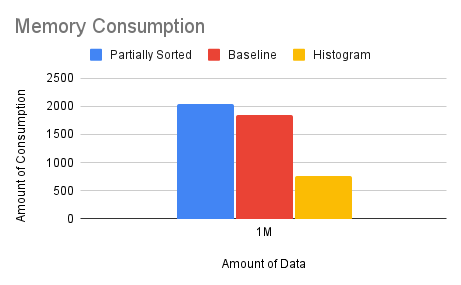
\includegraphics[width=100mm,scale=1]{Figures/MemoryPowerlaw.png}
    \caption{
     Results of Memory Consumption with Powerlaw Distribution Dataset 1M
    }
    \label{fig:MemoryPowerlaw}
\end{figure}
Our memory consumption test on the Powerlaw Distribution shows a similar trend to that of the Gaussian Distribution (Figure \ref{fig:MemoryPowerlaw}). The histogram outperforms both the baseline and partially sorted array in memory consumption. The histogram consumes less memory, making it more efficient for use in a static scenario where the data distribution is known. It is able to create fewer child nodes, utilizing the \textsf{gaps} efficiently.

On the other hand, the partially sorted array delays the creation of new nodes to amortize the cost. However, as the amount of data increases, it will eventually have to spend a significant amount of time rebuilding nodes recursively. This means that the number of nodes that need to be rebuilt will continue to increase as more data is added to the \learnindex.

Similarly, the baseline performs similarly to the partially sorted array. It does not make any assumptions about the data distribution, unlike the histogram, which creates more child nodes than the baseline.

\subsection{Lognormal Distribution}
\begin{figure}[H]
    \centering
    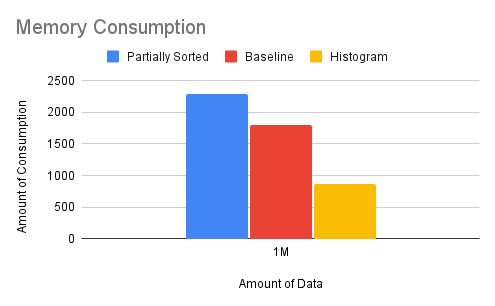
\includegraphics[width=100mm,scale=1]{Figures/MemoryLognormal.png}
    \caption{
     Results of Memory Consumption with Lognormal Distribution Dataset 1M
    }
    \label{fig:MemoryLognormal}
\end{figure}
The memory consumption test showed that the histogram outperformed the baseline and partially sorted \learnindex, which is consistent with the results from the Powerlaw Distribution (Figure \ref{fig:MemoryLognormal}). The histogram is able to maintain the distribution and gaps based on the data distribution, which allows it to have a lower average tree depth and consume less memory compared to the other two implementations.

On the other hand, the baseline only optimizes the keys based on the linear regression slope, which does not take into account the distribution of the data. As a result, it creates more child nodes and consumes more memory than the histogram. The partially sorted array delays the creation of new nodes to amortize the cost, but as the data becomes larger, it still needs to rebuild nodes recursively, resulting in more memory consumption.

Overall, the histogram is a more efficient implementation for static scenarios where the data distribution is known. Its ability to maintain gaps and distribution reduces the need for creating new child nodes and, thus, results in lower memory consumption.

\subsection{Real-World Dataset (Longitudes)}
\begin{figure}[H]
    \centering
    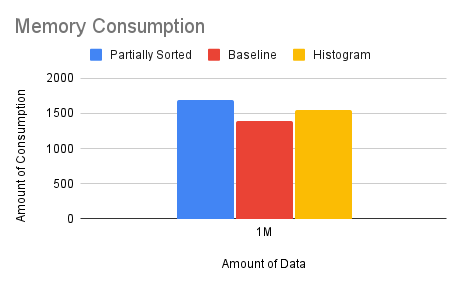
\includegraphics[width=100mm,scale=1]{Figures/MemoryLongitude.png}
    \caption{
     Results of Memory Consumption with Longitudes Distribution Dataset 1M
    }
    \label{fig:MemoryLongitude}
\end{figure}
However, for real-world scenarios where distribution is not known, the histogram performs worse than the baseline and is not able to capture the distribution of the data since the assumption is not valid for real-world data where distribution is known for newly insert keys (Figure \ref{fig:MemoryLongitude}). Since the histogram is not able to optimize based on the distribution, the histogram will cause more \conflict than the baseline which is expected and hence consume more memory. 

Similar to the histogram, the partially sorted method does not depend on any particular distribution. However, it defers resolving conflicts until all available empty spaces are filled, at which point it creates new child nodes. The results indicate that the partially sorted method performs slightly better than the histogram technique because it delays creating new nodes until a later stage. However, when there is a larger amount of data in the tree, the partially sorted method does consume more resources than the histogram. This is because it waits until the current node is completely filled before recursively rebuilding it, which uses up more memory.

When dealing with real-world datasets, it is better to use the baseline approach if memory consumption is a top priority. This method is highly adaptable and generally produces better outcomes than the histogram and partially sorted techniques. Nevertheless, if the data distribution is familiar, the histogram approach can be fine-tuned to better fit the data. 

\section{Number of New Node Creation / Tree depth}
In this section, we investigate the performance of three different \learnindex implementations, namely the histogram, partially sorted, and baseline, in terms of the number of new node creations or \conflict when using different datasets.

The number of \conflict is crucial in evaluating the performance of \learnindex algorithms, especially in dynamic scenarios, where the data distribution can change over time. For instance, when a new key is inserted into the tree, it may cause \conflict and result in new node creations to maintain the performance of the algorithm. Therefore, measuring the number of \conflict can provide insights into how well each \learnindex implementation adapts to changes in the data distribution.


We tested the three algorithms by performing bulk loading of one million to twenty million. After performing bulk loading we perform insertion for another one million to twenty million to test the trend and new node creation on different algorithms. Basically, we bulk load fifty percent of the keys in and insert another fifty percent later to perform the experiment, which means that one million will have two million in the tree. 


\subsection{Gaussian Distribution}
\begin{figure}[H]
    \centering
    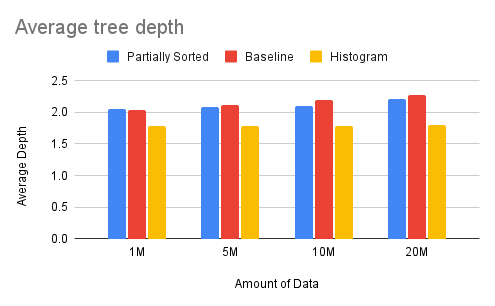
\includegraphics[width=100mm,scale=1]{Figures/AVGTD-Gau.png}
    \caption{
     Results of Average tree depth after a number of insertions (Gaussian)
    }
    \label{fig:AverageTreeDepthGau}
\end{figure}

From the results Figure \ref{fig:AverageTreeDepthGau}, we found that the histogram performs better on the average tree depth compared to the other two algorithms. Furthermore it has lesser \conflict number (new node creation) compared to partially sorted and baseline. This is because histogram is able to capture distributions of the data while partially sorted only delays \conflict until running out of space. This is inline with other experiments from previous sections. As lesser average tree depth improve operations performance as all of the operations are bounded by the height of the tree. For example, if we are able to reduce the depth of the tree, we will be able to reduce the time to perform read and write operations.

On the other hand, from result Figure \ref{fig:AverageTreeDepthGau}, the partially performs similarly to the baseline due, this is because the main idea of partially sorted is to store keys after the predicted position and reduce the number of new node creation. However, this is only delaying creating new node until later which will still be incured. This results inline with the operation experiments above as the amount of tree depth increase, the longer time it takes to perform read and write operation. Furthermore, the poor result on operations for partially sorted is due to the cost of recusively rebuilding the keys to be sorted.


In addition, the baseline performs worse than the histogram as the baseline implementation does not consider the data distribution, resulting in a higher number of average tree depth as it fails to optimize key positioning. From the results Figure \ref{fig:AverageTreeDepthGau}, can see that the baseline has higher average tree depth compared to histogram, which is inline with operations performance as histogram outperform the baseline in operations as well due to having lesser depth to traverse.



\subsection{Powerlaw Distribution}
\begin{figure}[H]
    \centering
    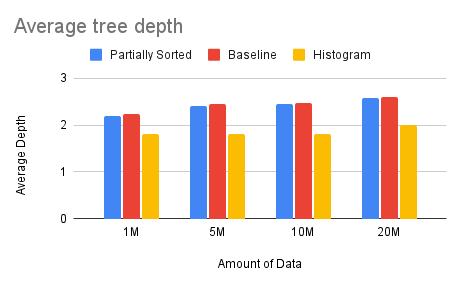
\includegraphics[width=100mm,scale=1]{Figures/AVGTD-Pow.png}
    \caption{
     Results of Average tree depth after a number of insertions (Powerlaw)
    }
    \label{fig:AverageTreeDepthPow}
\end{figure}
The result tested on Powerlaw distribution is not different from the Gaussian distribution (Figure \ref{fig:AverageTreeDepthPow}) where the histogram is able to outperforms both algorithm. This is because histogram can capture the distribution of the data and make use of the upper nodes gaps while the baseline just create new nodes whenever there is a \conflict and only wait until the next branch pruning (or adjustment) to occupy the upper nodes. 


Furthermore, partially sorted performs on par with the baseline as it only delays the new node creation until $\epsilon$ spaces runs out. From the result Figure \ref{fig:AverageTreeDepthPow}, we can see that the trend of average tree depth slowly increasing as more keys inserted in the tree. Even though the amount of data increase almost $10\times$, but the average tree depth does not increase much because of the branch pruning method that helps to reduce the amount of tree depth. However, we can see that the amount of average tree depth still increase for both partially sorted and baseline. While histogram is able to take advantage of the empty gaps in the upper node, which will create lesser new child node.

\subsection{Lognormal Distribution}
The result on Lognormal Distribution follows the same trend as previous distributions (Figure \ref{fig:AverageTreeDepthLog}). However the main difference from the previous test is that the baseline seem to have lesser average tree depth from five million to ten million, this is because when it reaches a condition, the baseline will trigger branch pruning which reduces the tree depth. 
\begin{figure}[H]
    \centering
    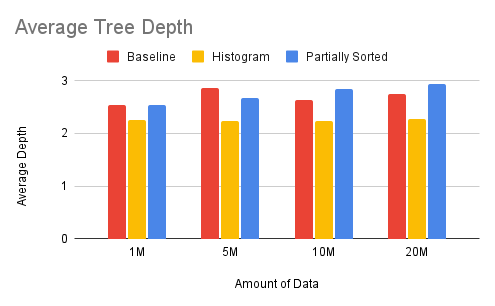
\includegraphics[width=100mm,scale=1]{Figures/AVGTD-Log.png}
    \caption{
     Results of Average tree depth after a number of insertions (Lognormal)
    }
    \label{fig:AverageTreeDepthLog}
\end{figure}

For histogram, we can see a similar trend where the histogram able to maintain the average tree height throughout the data increases. Which is inline with the result of insertion and search operations where it outperforms the baseline and partially sorted array. If it is able to make use of the upper nodes gaps, it will not need to wait until the branch pruning to make use of the available gaps in the upper nodes. 

\subsection{Real-World Dataset (Longitudes)}

On the other hand, the results on dynamic scenario (Figure \ref{fig:AverageTreeDepthLong}) shows that the baseline outperforms histogram and the partially sorted. Based from the result Figure \ref{fig:AverageTreeDepthLong}, we can see the baseline is able to make use of the gaps to insert and does not increase in the average depth while histogram does not perform when it comes to dynamic scenario as histogram can not capture the distribution which is crucial for histogram to work well. This results inline with the previous test on operations where baseline is able to out shine the histogram and partially sorted. This is because the search operation is only bounded by $O(h)$ where h is the height of the tree. This mean that reducing the amount of average tree depth will make the performance of the operations faster. 
Furthermore, the partially sorted perform similarly to both histogram and the baseline, as it make uses of the gaps by inserted keys after the predicted position which delays the new node creation, thus having lesser depth. 
\begin{figure}[H]
    \centering
    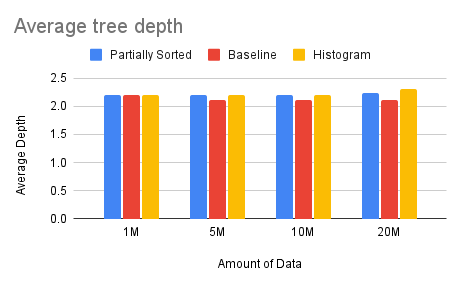
\includegraphics[width=100mm,scale=1]{Figures/AVGTD-Long.png}
    \caption{
     Results of Average tree depth after a number of insertions (Longitudes)
    }
    \label{fig:AverageTreeDepthLong}
\end{figure}
However this does not inline with the operations performance, this is because the operation performance of the partially sorted is bounded not just by the height of the tree, but also $\epsilon$ spaces. Which is similar to the section on \nameref{partialsortedtheory} where we mentioned that the time complexity of the operations is $O(\epsilon + \log N)$



\section{Evaluation Summary}
In this section, we have compared the performance of three learned index algorithms: baseline, histogram, and partially sorted. Our testing showed that the histogram implementation outperforms the baseline in operations such as insertion, deletion, and query when the distribution is static, and new keys follow the same distribution. This is due to the histogram's ability to minimize the height of the tree by grouping keys with similar values into a single bin, leading to faster traversal times.

In addition, measuring the number of \conflict can provide valuable insights into the performance of \learnindex algorithms in dynamic scenarios. The histogram implementation performs the best in terms of the number of \conflict, followed by the partially sorted implementation, while the baseline implementation performs the worst on the static scenario. On the other hand, the baseline outperforms the histogram and the partially sorted on the dynamic scenario. If the data distribution is known, histogram seems to be a better fit to optimize the gaps while performing faster on operations. If the data distribution is not known, baseline seem to perform better as it generalize to fit in many scenarios. Furthermore, the partially sorted still need more experiments and improve as the searches is still bounded by the extra search spaces after the predicted position which makes it slower during read and write operations.

However, our testing also revealed that the histogram implementation needed further exploration to improve its performance in real-world scenarios where data is not static and can change over time. This is an area where the partially sorted algorithm falls short, as it requires extra computation that causes operations to slow down as the data increases in the tree.

In conclusion, the choice of the learned index algorithm depends on the characteristics of the dataset being indexed and the expected usage patterns. For static distributions, the histogram algorithm offers the best performance, while the partially sorted algorithm may be more suitable for dynamic data. Nonetheless, further research is needed to explore the potential of these algorithms in more diverse scenarios and to develop more advanced learned index structures that can handle more complex data distributions.